%%% This is a knitr document, not regular Sweave
%%% http://yihui.name/knitr/

\documentclass[]{beamer}
\usepackage{graphicx, color}
\newcommand{\hlnumber}[1]{\textcolor[rgb]{0,0,0}{#1}}%
\newcommand{\hlfunctioncall}[1]{\textcolor[rgb]{.5,0,.33}{\textbf{#1}}}%
\newcommand{\hlstring}[1]{\textcolor[rgb]{.6,.6,1}{#1}}%
\newcommand{\hlkeyword}[1]{\textbf{#1}}%
\newcommand{\hlargument}[1]{\textcolor[rgb]{.69,.25,.02}{#1}}%
\newcommand{\hlcomment}[1]{\textcolor[rgb]{.18,.6,.34}{#1}}%
\newcommand{\hlroxygencomment}[1]{\textcolor[rgb]{.44,.48,.7}{#1}}%
\newcommand{\hlformalargs}[1]{\hlargument{#1}}%
\newcommand{\hleqformalargs}[1]{\hlargument{#1}}%
\newcommand{\hlassignement}[1]{\textbf{#1}}%
\newcommand{\hlpackage}[1]{\textcolor[rgb]{.59,.71,.145}{#1}}%
\newcommand{\hlslot}[1]{\textit{#1}}%
\newcommand{\hlsymbol}[1]{#1}%
\newcommand{\hlprompt}[1]{\textcolor[rgb]{.5,.5,.5}{#1}}%

\usepackage{color}%
 
\newsavebox{\hlnormalsizeboxclosebrace}%
\newsavebox{\hlnormalsizeboxopenbrace}%
\newsavebox{\hlnormalsizeboxbackslash}%
\newsavebox{\hlnormalsizeboxlessthan}%
\newsavebox{\hlnormalsizeboxgreaterthan}%
\newsavebox{\hlnormalsizeboxdollar}%
\newsavebox{\hlnormalsizeboxunderscore}%
\newsavebox{\hlnormalsizeboxand}%
\newsavebox{\hlnormalsizeboxhash}%
\newsavebox{\hlnormalsizeboxat}%
\newsavebox{\hlnormalsizeboxpercent}% 
\newsavebox{\hlnormalsizeboxhat}%
\newsavebox{\hlnormalsizeboxsinglequote}%
\newsavebox{\hlnormalsizeboxbacktick}%

\setbox\hlnormalsizeboxopenbrace=\hbox{\begin{normalsize}\verb.{.\end{normalsize}}%
\setbox\hlnormalsizeboxclosebrace=\hbox{\begin{normalsize}\verb.}.\end{normalsize}}%
\setbox\hlnormalsizeboxlessthan=\hbox{\begin{normalsize}\verb.<.\end{normalsize}}%
\setbox\hlnormalsizeboxdollar=\hbox{\begin{normalsize}\verb.$.\end{normalsize}}%
\setbox\hlnormalsizeboxunderscore=\hbox{\begin{normalsize}\verb._.\end{normalsize}}%
\setbox\hlnormalsizeboxand=\hbox{\begin{normalsize}\verb.&.\end{normalsize}}%
\setbox\hlnormalsizeboxhash=\hbox{\begin{normalsize}\verb.#.\end{normalsize}}%
\setbox\hlnormalsizeboxat=\hbox{\begin{normalsize}\verb.@.\end{normalsize}}%
\setbox\hlnormalsizeboxbackslash=\hbox{\begin{normalsize}\verb.\.\end{normalsize}}%
\setbox\hlnormalsizeboxgreaterthan=\hbox{\begin{normalsize}\verb.>.\end{normalsize}}%
\setbox\hlnormalsizeboxpercent=\hbox{\begin{normalsize}\verb.%.\end{normalsize}}%
\setbox\hlnormalsizeboxhat=\hbox{\begin{normalsize}\verb.^.\end{normalsize}}%
\setbox\hlnormalsizeboxsinglequote=\hbox{\begin{normalsize}\verb.'.\end{normalsize}}%
\setbox\hlnormalsizeboxbacktick=\hbox{\begin{normalsize}\verb.`.\end{normalsize}}%
\setbox\hlnormalsizeboxhat=\hbox{\begin{normalsize}\verb.^.\end{normalsize}}%



\newsavebox{\hltinyboxclosebrace}%
\newsavebox{\hltinyboxopenbrace}%
\newsavebox{\hltinyboxbackslash}%
\newsavebox{\hltinyboxlessthan}%
\newsavebox{\hltinyboxgreaterthan}%
\newsavebox{\hltinyboxdollar}%
\newsavebox{\hltinyboxunderscore}%
\newsavebox{\hltinyboxand}%
\newsavebox{\hltinyboxhash}%
\newsavebox{\hltinyboxat}%
\newsavebox{\hltinyboxpercent}% 
\newsavebox{\hltinyboxhat}%
\newsavebox{\hltinyboxsinglequote}%
\newsavebox{\hltinyboxbacktick}%

\setbox\hltinyboxopenbrace=\hbox{\begin{tiny}\verb.{.\end{tiny}}%
\setbox\hltinyboxclosebrace=\hbox{\begin{tiny}\verb.}.\end{tiny}}%
\setbox\hltinyboxlessthan=\hbox{\begin{tiny}\verb.<.\end{tiny}}%
\setbox\hltinyboxdollar=\hbox{\begin{tiny}\verb.$.\end{tiny}}%
\setbox\hltinyboxunderscore=\hbox{\begin{tiny}\verb._.\end{tiny}}%
\setbox\hltinyboxand=\hbox{\begin{tiny}\verb.&.\end{tiny}}%
\setbox\hltinyboxhash=\hbox{\begin{tiny}\verb.#.\end{tiny}}%
\setbox\hltinyboxat=\hbox{\begin{tiny}\verb.@.\end{tiny}}%
\setbox\hltinyboxbackslash=\hbox{\begin{tiny}\verb.\.\end{tiny}}%
\setbox\hltinyboxgreaterthan=\hbox{\begin{tiny}\verb.>.\end{tiny}}%
\setbox\hltinyboxpercent=\hbox{\begin{tiny}\verb.%.\end{tiny}}%
\setbox\hltinyboxhat=\hbox{\begin{tiny}\verb.^.\end{tiny}}%
\setbox\hltinyboxsinglequote=\hbox{\begin{tiny}\verb.'.\end{tiny}}%
\setbox\hltinyboxbacktick=\hbox{\begin{tiny}\verb.`.\end{tiny}}%
\setbox\hltinyboxhat=\hbox{\begin{tiny}\verb.^.\end{tiny}}%



\newsavebox{\hlscriptsizeboxclosebrace}%
\newsavebox{\hlscriptsizeboxopenbrace}%
\newsavebox{\hlscriptsizeboxbackslash}%
\newsavebox{\hlscriptsizeboxlessthan}%
\newsavebox{\hlscriptsizeboxgreaterthan}%
\newsavebox{\hlscriptsizeboxdollar}%
\newsavebox{\hlscriptsizeboxunderscore}%
\newsavebox{\hlscriptsizeboxand}%
\newsavebox{\hlscriptsizeboxhash}%
\newsavebox{\hlscriptsizeboxat}%
\newsavebox{\hlscriptsizeboxpercent}% 
\newsavebox{\hlscriptsizeboxhat}%
\newsavebox{\hlscriptsizeboxsinglequote}%
\newsavebox{\hlscriptsizeboxbacktick}%

\setbox\hlscriptsizeboxopenbrace=\hbox{\begin{scriptsize}\verb.{.\end{scriptsize}}%
\setbox\hlscriptsizeboxclosebrace=\hbox{\begin{scriptsize}\verb.}.\end{scriptsize}}%
\setbox\hlscriptsizeboxlessthan=\hbox{\begin{scriptsize}\verb.<.\end{scriptsize}}%
\setbox\hlscriptsizeboxdollar=\hbox{\begin{scriptsize}\verb.$.\end{scriptsize}}%
\setbox\hlscriptsizeboxunderscore=\hbox{\begin{scriptsize}\verb._.\end{scriptsize}}%
\setbox\hlscriptsizeboxand=\hbox{\begin{scriptsize}\verb.&.\end{scriptsize}}%
\setbox\hlscriptsizeboxhash=\hbox{\begin{scriptsize}\verb.#.\end{scriptsize}}%
\setbox\hlscriptsizeboxat=\hbox{\begin{scriptsize}\verb.@.\end{scriptsize}}%
\setbox\hlscriptsizeboxbackslash=\hbox{\begin{scriptsize}\verb.\.\end{scriptsize}}%
\setbox\hlscriptsizeboxgreaterthan=\hbox{\begin{scriptsize}\verb.>.\end{scriptsize}}%
\setbox\hlscriptsizeboxpercent=\hbox{\begin{scriptsize}\verb.%.\end{scriptsize}}%
\setbox\hlscriptsizeboxhat=\hbox{\begin{scriptsize}\verb.^.\end{scriptsize}}%
\setbox\hlscriptsizeboxsinglequote=\hbox{\begin{scriptsize}\verb.'.\end{scriptsize}}%
\setbox\hlscriptsizeboxbacktick=\hbox{\begin{scriptsize}\verb.`.\end{scriptsize}}%
\setbox\hlscriptsizeboxhat=\hbox{\begin{scriptsize}\verb.^.\end{scriptsize}}%



\newsavebox{\hlfootnotesizeboxclosebrace}%
\newsavebox{\hlfootnotesizeboxopenbrace}%
\newsavebox{\hlfootnotesizeboxbackslash}%
\newsavebox{\hlfootnotesizeboxlessthan}%
\newsavebox{\hlfootnotesizeboxgreaterthan}%
\newsavebox{\hlfootnotesizeboxdollar}%
\newsavebox{\hlfootnotesizeboxunderscore}%
\newsavebox{\hlfootnotesizeboxand}%
\newsavebox{\hlfootnotesizeboxhash}%
\newsavebox{\hlfootnotesizeboxat}%
\newsavebox{\hlfootnotesizeboxpercent}% 
\newsavebox{\hlfootnotesizeboxhat}%
\newsavebox{\hlfootnotesizeboxsinglequote}%
\newsavebox{\hlfootnotesizeboxbacktick}%

\setbox\hlfootnotesizeboxopenbrace=\hbox{\begin{footnotesize}\verb.{.\end{footnotesize}}%
\setbox\hlfootnotesizeboxclosebrace=\hbox{\begin{footnotesize}\verb.}.\end{footnotesize}}%
\setbox\hlfootnotesizeboxlessthan=\hbox{\begin{footnotesize}\verb.<.\end{footnotesize}}%
\setbox\hlfootnotesizeboxdollar=\hbox{\begin{footnotesize}\verb.$.\end{footnotesize}}%
\setbox\hlfootnotesizeboxunderscore=\hbox{\begin{footnotesize}\verb._.\end{footnotesize}}%
\setbox\hlfootnotesizeboxand=\hbox{\begin{footnotesize}\verb.&.\end{footnotesize}}%
\setbox\hlfootnotesizeboxhash=\hbox{\begin{footnotesize}\verb.#.\end{footnotesize}}%
\setbox\hlfootnotesizeboxat=\hbox{\begin{footnotesize}\verb.@.\end{footnotesize}}%
\setbox\hlfootnotesizeboxbackslash=\hbox{\begin{footnotesize}\verb.\.\end{footnotesize}}%
\setbox\hlfootnotesizeboxgreaterthan=\hbox{\begin{footnotesize}\verb.>.\end{footnotesize}}%
\setbox\hlfootnotesizeboxpercent=\hbox{\begin{footnotesize}\verb.%.\end{footnotesize}}%
\setbox\hlfootnotesizeboxhat=\hbox{\begin{footnotesize}\verb.^.\end{footnotesize}}%
\setbox\hlfootnotesizeboxsinglequote=\hbox{\begin{footnotesize}\verb.'.\end{footnotesize}}%
\setbox\hlfootnotesizeboxbacktick=\hbox{\begin{footnotesize}\verb.`.\end{footnotesize}}%
\setbox\hlfootnotesizeboxhat=\hbox{\begin{footnotesize}\verb.^.\end{footnotesize}}%



\newsavebox{\hlsmallboxclosebrace}%
\newsavebox{\hlsmallboxopenbrace}%
\newsavebox{\hlsmallboxbackslash}%
\newsavebox{\hlsmallboxlessthan}%
\newsavebox{\hlsmallboxgreaterthan}%
\newsavebox{\hlsmallboxdollar}%
\newsavebox{\hlsmallboxunderscore}%
\newsavebox{\hlsmallboxand}%
\newsavebox{\hlsmallboxhash}%
\newsavebox{\hlsmallboxat}%
\newsavebox{\hlsmallboxpercent}% 
\newsavebox{\hlsmallboxhat}%
\newsavebox{\hlsmallboxsinglequote}%
\newsavebox{\hlsmallboxbacktick}%

\setbox\hlsmallboxopenbrace=\hbox{\begin{small}\verb.{.\end{small}}%
\setbox\hlsmallboxclosebrace=\hbox{\begin{small}\verb.}.\end{small}}%
\setbox\hlsmallboxlessthan=\hbox{\begin{small}\verb.<.\end{small}}%
\setbox\hlsmallboxdollar=\hbox{\begin{small}\verb.$.\end{small}}%
\setbox\hlsmallboxunderscore=\hbox{\begin{small}\verb._.\end{small}}%
\setbox\hlsmallboxand=\hbox{\begin{small}\verb.&.\end{small}}%
\setbox\hlsmallboxhash=\hbox{\begin{small}\verb.#.\end{small}}%
\setbox\hlsmallboxat=\hbox{\begin{small}\verb.@.\end{small}}%
\setbox\hlsmallboxbackslash=\hbox{\begin{small}\verb.\.\end{small}}%
\setbox\hlsmallboxgreaterthan=\hbox{\begin{small}\verb.>.\end{small}}%
\setbox\hlsmallboxpercent=\hbox{\begin{small}\verb.%.\end{small}}%
\setbox\hlsmallboxhat=\hbox{\begin{small}\verb.^.\end{small}}%
\setbox\hlsmallboxsinglequote=\hbox{\begin{small}\verb.'.\end{small}}%
\setbox\hlsmallboxbacktick=\hbox{\begin{small}\verb.`.\end{small}}%
\setbox\hlsmallboxhat=\hbox{\begin{small}\verb.^.\end{small}}%



\newsavebox{\hllargeboxclosebrace}%
\newsavebox{\hllargeboxopenbrace}%
\newsavebox{\hllargeboxbackslash}%
\newsavebox{\hllargeboxlessthan}%
\newsavebox{\hllargeboxgreaterthan}%
\newsavebox{\hllargeboxdollar}%
\newsavebox{\hllargeboxunderscore}%
\newsavebox{\hllargeboxand}%
\newsavebox{\hllargeboxhash}%
\newsavebox{\hllargeboxat}%
\newsavebox{\hllargeboxpercent}% 
\newsavebox{\hllargeboxhat}%
\newsavebox{\hllargeboxsinglequote}%
\newsavebox{\hllargeboxbacktick}%

\setbox\hllargeboxopenbrace=\hbox{\begin{large}\verb.{.\end{large}}%
\setbox\hllargeboxclosebrace=\hbox{\begin{large}\verb.}.\end{large}}%
\setbox\hllargeboxlessthan=\hbox{\begin{large}\verb.<.\end{large}}%
\setbox\hllargeboxdollar=\hbox{\begin{large}\verb.$.\end{large}}%
\setbox\hllargeboxunderscore=\hbox{\begin{large}\verb._.\end{large}}%
\setbox\hllargeboxand=\hbox{\begin{large}\verb.&.\end{large}}%
\setbox\hllargeboxhash=\hbox{\begin{large}\verb.#.\end{large}}%
\setbox\hllargeboxat=\hbox{\begin{large}\verb.@.\end{large}}%
\setbox\hllargeboxbackslash=\hbox{\begin{large}\verb.\.\end{large}}%
\setbox\hllargeboxgreaterthan=\hbox{\begin{large}\verb.>.\end{large}}%
\setbox\hllargeboxpercent=\hbox{\begin{large}\verb.%.\end{large}}%
\setbox\hllargeboxhat=\hbox{\begin{large}\verb.^.\end{large}}%
\setbox\hllargeboxsinglequote=\hbox{\begin{large}\verb.'.\end{large}}%
\setbox\hllargeboxbacktick=\hbox{\begin{large}\verb.`.\end{large}}%
\setbox\hllargeboxhat=\hbox{\begin{large}\verb.^.\end{large}}%



\newsavebox{\hlLargeboxclosebrace}%
\newsavebox{\hlLargeboxopenbrace}%
\newsavebox{\hlLargeboxbackslash}%
\newsavebox{\hlLargeboxlessthan}%
\newsavebox{\hlLargeboxgreaterthan}%
\newsavebox{\hlLargeboxdollar}%
\newsavebox{\hlLargeboxunderscore}%
\newsavebox{\hlLargeboxand}%
\newsavebox{\hlLargeboxhash}%
\newsavebox{\hlLargeboxat}%
\newsavebox{\hlLargeboxpercent}% 
\newsavebox{\hlLargeboxhat}%
\newsavebox{\hlLargeboxsinglequote}%
\newsavebox{\hlLargeboxbacktick}%

\setbox\hlLargeboxopenbrace=\hbox{\begin{Large}\verb.{.\end{Large}}%
\setbox\hlLargeboxclosebrace=\hbox{\begin{Large}\verb.}.\end{Large}}%
\setbox\hlLargeboxlessthan=\hbox{\begin{Large}\verb.<.\end{Large}}%
\setbox\hlLargeboxdollar=\hbox{\begin{Large}\verb.$.\end{Large}}%
\setbox\hlLargeboxunderscore=\hbox{\begin{Large}\verb._.\end{Large}}%
\setbox\hlLargeboxand=\hbox{\begin{Large}\verb.&.\end{Large}}%
\setbox\hlLargeboxhash=\hbox{\begin{Large}\verb.#.\end{Large}}%
\setbox\hlLargeboxat=\hbox{\begin{Large}\verb.@.\end{Large}}%
\setbox\hlLargeboxbackslash=\hbox{\begin{Large}\verb.\.\end{Large}}%
\setbox\hlLargeboxgreaterthan=\hbox{\begin{Large}\verb.>.\end{Large}}%
\setbox\hlLargeboxpercent=\hbox{\begin{Large}\verb.%.\end{Large}}%
\setbox\hlLargeboxhat=\hbox{\begin{Large}\verb.^.\end{Large}}%
\setbox\hlLargeboxsinglequote=\hbox{\begin{Large}\verb.'.\end{Large}}%
\setbox\hlLargeboxbacktick=\hbox{\begin{Large}\verb.`.\end{Large}}%
\setbox\hlLargeboxhat=\hbox{\begin{Large}\verb.^.\end{Large}}%



\newsavebox{\hlLARGEboxclosebrace}%
\newsavebox{\hlLARGEboxopenbrace}%
\newsavebox{\hlLARGEboxbackslash}%
\newsavebox{\hlLARGEboxlessthan}%
\newsavebox{\hlLARGEboxgreaterthan}%
\newsavebox{\hlLARGEboxdollar}%
\newsavebox{\hlLARGEboxunderscore}%
\newsavebox{\hlLARGEboxand}%
\newsavebox{\hlLARGEboxhash}%
\newsavebox{\hlLARGEboxat}%
\newsavebox{\hlLARGEboxpercent}% 
\newsavebox{\hlLARGEboxhat}%
\newsavebox{\hlLARGEboxsinglequote}%
\newsavebox{\hlLARGEboxbacktick}%

\setbox\hlLARGEboxopenbrace=\hbox{\begin{LARGE}\verb.{.\end{LARGE}}%
\setbox\hlLARGEboxclosebrace=\hbox{\begin{LARGE}\verb.}.\end{LARGE}}%
\setbox\hlLARGEboxlessthan=\hbox{\begin{LARGE}\verb.<.\end{LARGE}}%
\setbox\hlLARGEboxdollar=\hbox{\begin{LARGE}\verb.$.\end{LARGE}}%
\setbox\hlLARGEboxunderscore=\hbox{\begin{LARGE}\verb._.\end{LARGE}}%
\setbox\hlLARGEboxand=\hbox{\begin{LARGE}\verb.&.\end{LARGE}}%
\setbox\hlLARGEboxhash=\hbox{\begin{LARGE}\verb.#.\end{LARGE}}%
\setbox\hlLARGEboxat=\hbox{\begin{LARGE}\verb.@.\end{LARGE}}%
\setbox\hlLARGEboxbackslash=\hbox{\begin{LARGE}\verb.\.\end{LARGE}}%
\setbox\hlLARGEboxgreaterthan=\hbox{\begin{LARGE}\verb.>.\end{LARGE}}%
\setbox\hlLARGEboxpercent=\hbox{\begin{LARGE}\verb.%.\end{LARGE}}%
\setbox\hlLARGEboxhat=\hbox{\begin{LARGE}\verb.^.\end{LARGE}}%
\setbox\hlLARGEboxsinglequote=\hbox{\begin{LARGE}\verb.'.\end{LARGE}}%
\setbox\hlLARGEboxbacktick=\hbox{\begin{LARGE}\verb.`.\end{LARGE}}%
\setbox\hlLARGEboxhat=\hbox{\begin{LARGE}\verb.^.\end{LARGE}}%



\newsavebox{\hlhugeboxclosebrace}%
\newsavebox{\hlhugeboxopenbrace}%
\newsavebox{\hlhugeboxbackslash}%
\newsavebox{\hlhugeboxlessthan}%
\newsavebox{\hlhugeboxgreaterthan}%
\newsavebox{\hlhugeboxdollar}%
\newsavebox{\hlhugeboxunderscore}%
\newsavebox{\hlhugeboxand}%
\newsavebox{\hlhugeboxhash}%
\newsavebox{\hlhugeboxat}%
\newsavebox{\hlhugeboxpercent}% 
\newsavebox{\hlhugeboxhat}%
\newsavebox{\hlhugeboxsinglequote}%
\newsavebox{\hlhugeboxbacktick}%

\setbox\hlhugeboxopenbrace=\hbox{\begin{huge}\verb.{.\end{huge}}%
\setbox\hlhugeboxclosebrace=\hbox{\begin{huge}\verb.}.\end{huge}}%
\setbox\hlhugeboxlessthan=\hbox{\begin{huge}\verb.<.\end{huge}}%
\setbox\hlhugeboxdollar=\hbox{\begin{huge}\verb.$.\end{huge}}%
\setbox\hlhugeboxunderscore=\hbox{\begin{huge}\verb._.\end{huge}}%
\setbox\hlhugeboxand=\hbox{\begin{huge}\verb.&.\end{huge}}%
\setbox\hlhugeboxhash=\hbox{\begin{huge}\verb.#.\end{huge}}%
\setbox\hlhugeboxat=\hbox{\begin{huge}\verb.@.\end{huge}}%
\setbox\hlhugeboxbackslash=\hbox{\begin{huge}\verb.\.\end{huge}}%
\setbox\hlhugeboxgreaterthan=\hbox{\begin{huge}\verb.>.\end{huge}}%
\setbox\hlhugeboxpercent=\hbox{\begin{huge}\verb.%.\end{huge}}%
\setbox\hlhugeboxhat=\hbox{\begin{huge}\verb.^.\end{huge}}%
\setbox\hlhugeboxsinglequote=\hbox{\begin{huge}\verb.'.\end{huge}}%
\setbox\hlhugeboxbacktick=\hbox{\begin{huge}\verb.`.\end{huge}}%
\setbox\hlhugeboxhat=\hbox{\begin{huge}\verb.^.\end{huge}}%



\newsavebox{\hlHugeboxclosebrace}%
\newsavebox{\hlHugeboxopenbrace}%
\newsavebox{\hlHugeboxbackslash}%
\newsavebox{\hlHugeboxlessthan}%
\newsavebox{\hlHugeboxgreaterthan}%
\newsavebox{\hlHugeboxdollar}%
\newsavebox{\hlHugeboxunderscore}%
\newsavebox{\hlHugeboxand}%
\newsavebox{\hlHugeboxhash}%
\newsavebox{\hlHugeboxat}%
\newsavebox{\hlHugeboxpercent}% 
\newsavebox{\hlHugeboxhat}%
\newsavebox{\hlHugeboxsinglequote}%
\newsavebox{\hlHugeboxbacktick}%

\setbox\hlHugeboxopenbrace=\hbox{\begin{Huge}\verb.{.\end{Huge}}%
\setbox\hlHugeboxclosebrace=\hbox{\begin{Huge}\verb.}.\end{Huge}}%
\setbox\hlHugeboxlessthan=\hbox{\begin{Huge}\verb.<.\end{Huge}}%
\setbox\hlHugeboxdollar=\hbox{\begin{Huge}\verb.$.\end{Huge}}%
\setbox\hlHugeboxunderscore=\hbox{\begin{Huge}\verb._.\end{Huge}}%
\setbox\hlHugeboxand=\hbox{\begin{Huge}\verb.&.\end{Huge}}%
\setbox\hlHugeboxhash=\hbox{\begin{Huge}\verb.#.\end{Huge}}%
\setbox\hlHugeboxat=\hbox{\begin{Huge}\verb.@.\end{Huge}}%
\setbox\hlHugeboxbackslash=\hbox{\begin{Huge}\verb.\.\end{Huge}}%
\setbox\hlHugeboxgreaterthan=\hbox{\begin{Huge}\verb.>.\end{Huge}}%
\setbox\hlHugeboxpercent=\hbox{\begin{Huge}\verb.%.\end{Huge}}%
\setbox\hlHugeboxhat=\hbox{\begin{Huge}\verb.^.\end{Huge}}%
\setbox\hlHugeboxsinglequote=\hbox{\begin{Huge}\verb.'.\end{Huge}}%
\setbox\hlHugeboxbacktick=\hbox{\begin{Huge}\verb.`.\end{Huge}}%
\setbox\hlHugeboxhat=\hbox{\begin{Huge}\verb.^.\end{Huge}}%
 

\def\urltilda{\kern -.15em\lower .7ex\hbox{\~{}}\kern .04em}%

\newcommand{\hlstd}[1]{\textcolor[rgb]{0,0,0}{#1}}%
\newcommand{\hlnum}[1]{\textcolor[rgb]{0.16,0.16,1}{#1}}
\newcommand{\hlesc}[1]{\textcolor[rgb]{1,0,1}{#1}}
\newcommand{\hlstr}[1]{\textcolor[rgb]{1,0,0}{#1}}
\newcommand{\hldstr}[1]{\textcolor[rgb]{0.51,0.51,0}{#1}}
\newcommand{\hlslc}[1]{\textcolor[rgb]{0.51,0.51,0.51}{\it{#1}}}
\newcommand{\hlcom}[1]{\textcolor[rgb]{0.51,0.51,0.51}{\it{#1}}}
\newcommand{\hldir}[1]{\textcolor[rgb]{0,0.51,0}{#1}}
\newcommand{\hlsym}[1]{\textcolor[rgb]{0,0,0}{#1}}
\newcommand{\hlline}[1]{\textcolor[rgb]{0.33,0.33,0.33}{#1}}
\newcommand{\hlkwa}[1]{\textcolor[rgb]{0,0,0}{\bf{#1}}}
\newcommand{\hlkwb}[1]{\textcolor[rgb]{0.51,0,0}{#1}}
\newcommand{\hlkwc}[1]{\textcolor[rgb]{0,0,0}{\bf{#1}}}
\newcommand{\hlkwd}[1]{\textcolor[rgb]{0,0,0.51}{#1}}

\definecolor{fgcolor}{rgb}{0,0,0}
\usepackage{framed}
\makeatletter
\newenvironment{kframe}{%
 \def\FrameCommand##1{\hskip\@totalleftmargin \hskip-\fboxsep
 \colorbox{shadecolor}{##1}\hskip-\fboxsep
     % There is no \@totalrightmargin, so:
     \hskip-\linewidth \hskip-\@totalleftmargin \hskip\columnwidth}%
 \MakeFramed {\advance\hsize-\width
   \@totalleftmargin\z@ \linewidth\hsize
   \@setminipage}}%
 {\par\unskip\endMakeFramed}
\makeatother

\definecolor{shadecolor}{rgb}{.97, .97, .97}
\newenvironment{knitrout}{}{} % an empty environment to be redefined in TeX

\newcommand{\SweaveOpts}[1]{}  % do not interfere with LaTeX
\newcommand{\SweaveInput}[1]{} % because they are not real TeX commands
\newcommand{\Sexpr}[1]{}       % will only be parsed by R

\usetheme{Singapore}
\usepackage{hyperref}
\usepackage{helvet}
\usepackage{graphicx}
\usepackage{tipa}
\usepackage{booktabs}
\usepackage{color}
\usepackage[normalem]{ulem}

\AtBeginSection[]
{
  \begin{frame}<beamer>{Outline}
    \tableofcontents[currentsection]
  \end{frame}
}

\ifdefined\knitrout
\renewenvironment{knitrout}{\begin{footnotesize}}{\end{footnotesize}}
\else
 \fi
	
\mode<presentation>
\title{Murders in Philadelphia}
\author{Josef Fruehwald}
%\date{}

	


\begin{document}
% very important to use option [fragile] for frames containing code output!

\begin{frame}
	\titlepage
\end{frame}

\section{The Data}


\begin{frame}
	\frametitle{The Data}

	The Philadelphia Inquirer has a Google Fusion table
	(\href{https://www.google.com/fusiontables/DataSource?snapid=S4035208e94}{\color{red} link}) 
	where they have compiled publicly available data from the Philadelphia Police Department on
	every murder in Philadelphia County between 1988 and 2011.
	
\end{frame}







\begin{frame}[fragile]
	\frametitle{The Data}
\begin{knitrout}
\definecolor{shadecolor}{rgb}{0.969, 0.969, 0.969}\color{fgcolor}\begin{kframe}
\begin{flushleft}
\ttfamily\noindent
\hlfunctioncall{nrow}\hlkeyword{(}\hlsymbol{philly}\hlkeyword{)}\mbox{}
\normalfont
\end{flushleft}
\begin{verbatim}
## [1] 8991
\end{verbatim}
\begin{flushleft}
\ttfamily\noindent
\hlfunctioncall{colnames}\hlkeyword{(}\hlsymbol{philly}\hlkeyword{)}\mbox{}
\normalfont
\end{flushleft}
\begin{verbatim}
##  [1] "date"      "lastname"  "firstname" "age"      
##  [5] "race"      "sex"       "cause"     "motive"   
##  [9] "weapon"    "time"     
\end{verbatim}
\end{kframe}
\end{knitrout}

\end{frame}

\begin{frame}[fragile]
	\frametitle{The Data}
\begin{knitrout}
\definecolor{shadecolor}{rgb}{0.969, 0.969, 0.969}\color{fgcolor}\begin{kframe}
\begin{flushleft}
\ttfamily\noindent
\hlfunctioncall{table}\hlkeyword{(}\hlfunctioncall{is.na}\hlkeyword{(}\hlsymbol{philly}\hlkeyword{\usebox{\hlnormalsizeboxdollar}}\hlsymbol{cause}\hlkeyword{)}\hlkeyword{)}\mbox{}
\normalfont
\end{flushleft}
\begin{verbatim}
## 
## FALSE  TRUE 
##  6931  2060 
\end{verbatim}
\begin{flushleft}
\ttfamily\noindent
\hlfunctioncall{table}\hlkeyword{(}\hlfunctioncall{is.na}\hlkeyword{(}\hlsymbol{philly}\hlkeyword{\usebox{\hlnormalsizeboxdollar}}\hlsymbol{motive}\hlkeyword{)}\hlkeyword{)}\mbox{}
\normalfont
\end{flushleft}
\begin{verbatim}
## 
## FALSE  TRUE 
##  6931  2060 
\end{verbatim}
\begin{flushleft}
\ttfamily\noindent
\hlfunctioncall{table}\hlkeyword{(}\hlfunctioncall{is.na}\hlkeyword{(}\hlsymbol{philly}\hlkeyword{\usebox{\hlnormalsizeboxdollar}}\hlsymbol{time}\hlkeyword{)}\hlkeyword{)}\mbox{}
\normalfont
\end{flushleft}
\begin{verbatim}
## 
## FALSE  TRUE 
##  2060  6931 
\end{verbatim}
\end{kframe}
\end{knitrout}

\end{frame}

\begin{frame}[fragile]
	\frametitle{The Data}
\begin{knitrout}
\definecolor{shadecolor}{rgb}{0.969, 0.969, 0.969}\color{fgcolor}\begin{kframe}
\begin{flushleft}
\ttfamily\noindent
\hlfunctioncall{library}\hlkeyword{(}\hlsymbol{reshape2}\hlkeyword{)}\hspace*{\fill}\\
\hlstd{}\hlfunctioncall{dcast}\hlkeyword{(}\hlsymbol{philly}\hlkeyword{,}{\ }\hlsymbol{race}{\ }\hlkeyword{\urltilda{}}{\ }\hlsymbol{weapon}\hlkeyword{)}\mbox{}
\normalfont
\end{flushleft}
\begin{verbatim}
##   race ARSON FIREARM HANDS KNIFE OTHER UNKNOWN
## 1    A     1      67     9    17     1       0
## 2    B    97    5610   467   676   171      15
## 3    H     2     269    31    36     3       0
## 4    I     0       2     0     0     0       0
## 5    M     0       1     0     0     0       0
## 6    O     5      50    12     8     0       0
## 7    W    35     951   214   171    63       5
## 8 <NA>     0       1     0     1     0       0
\end{verbatim}
\end{kframe}
\end{knitrout}

\end{frame}
















\begin{frame}[fragile]
	\frametitle{The Data}
	
	I've manipulated the data in my own way to include
	\begin{itemize}
		\item Month of year,
		\item month in Date format,
		\item year,
		\item a few different representations of the hour of day
		\item and the weekday.
	\end{itemize}
\end{frame}

\begin{frame}[fragile]
\frametitle{By Weekday}



\begin{knitrout}
\definecolor{shadecolor}{rgb}{0.969, 0.969, 0.969}\color{fgcolor}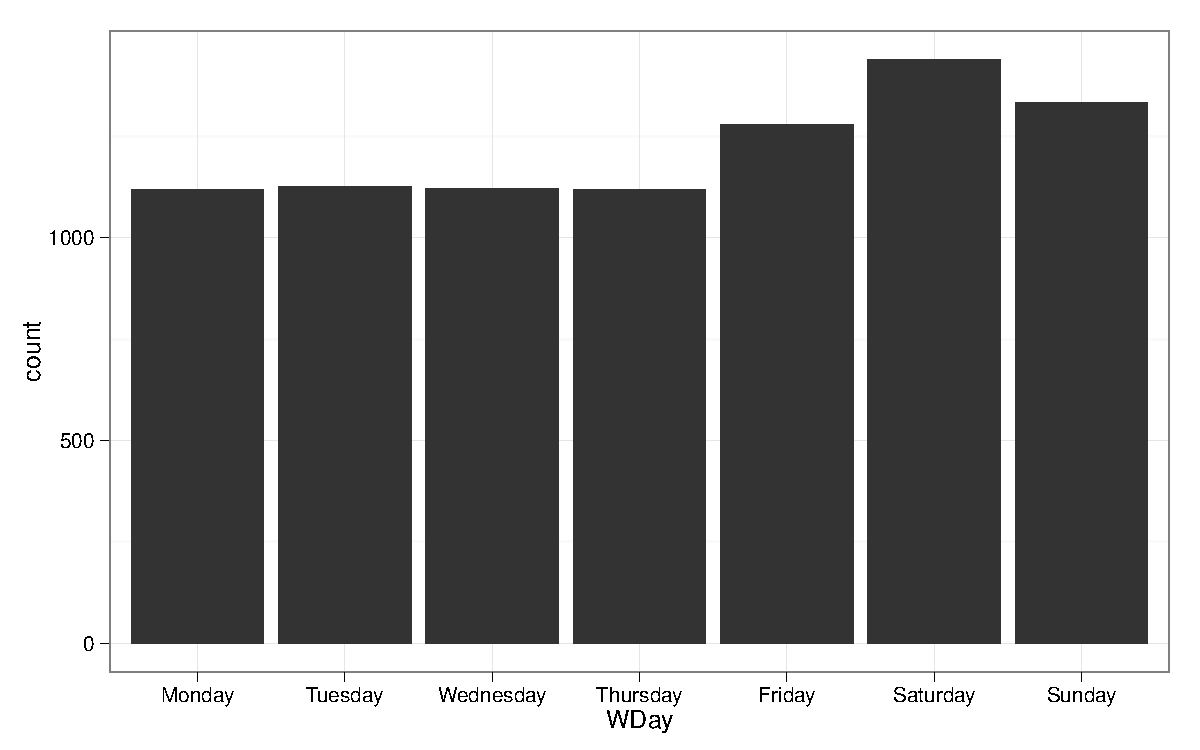
\includegraphics[width=\linewidth]{figures/murder-unnamed-chunk-3} 
\end{knitrout}


\end{frame}

\begin{frame}[fragile]
\frametitle{By Month}



\begin{knitrout}
\definecolor{shadecolor}{rgb}{0.969, 0.969, 0.969}\color{fgcolor}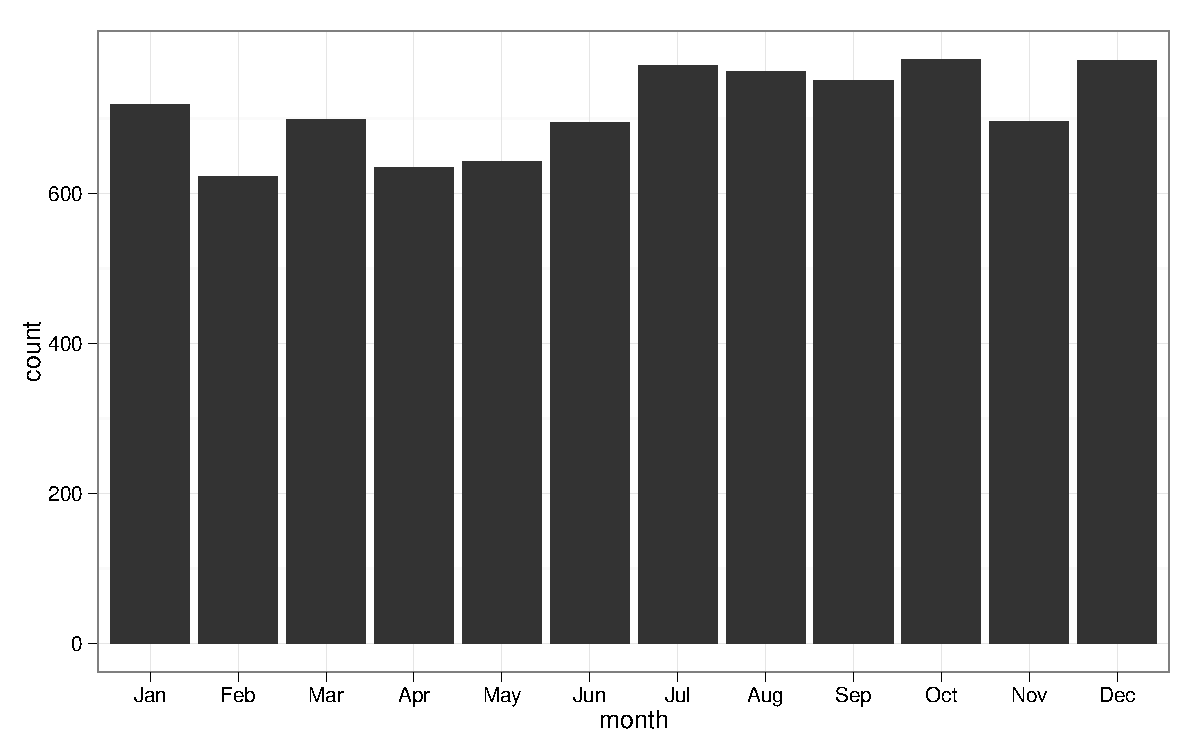
\includegraphics[width=\linewidth]{figures/murder-unnamed-chunk-4} 
\end{knitrout}

\end{frame}





\begin{frame}[fragile]
\frametitle{By Hour}



\begin{knitrout}
\definecolor{shadecolor}{rgb}{0.969, 0.969, 0.969}\color{fgcolor}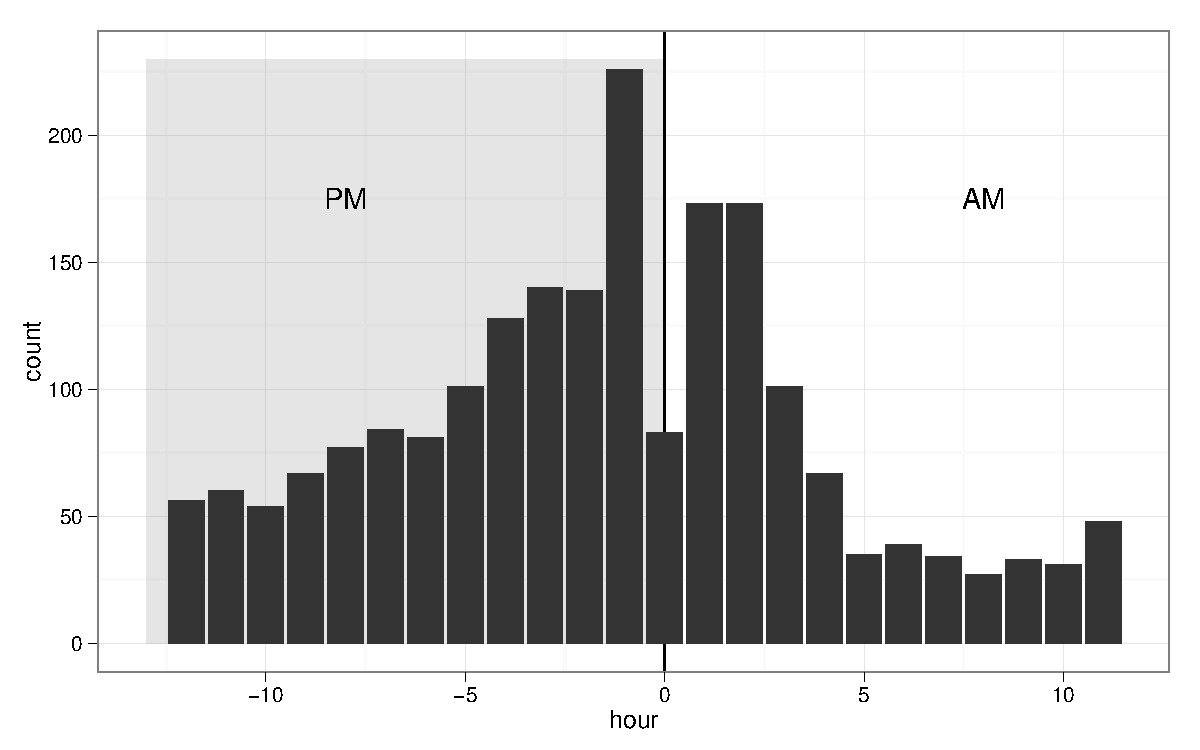
\includegraphics[width=\linewidth]{figures/murder-unnamed-chunk-6} 
\end{knitrout}

\end{frame}



\section{Two Philadelphias}



\begin{frame}[fragile]
\frametitle{Two Philadelphias}
\begin{knitrout}
\definecolor{shadecolor}{rgb}{0.969, 0.969, 0.969}\color{fgcolor}\begin{kframe}
\begin{flushleft}
\ttfamily\noindent
\hlsymbol{philly.bw}{\ }\hlassignement{\usebox{\hlnormalsizeboxlessthan}-}{\ }\hlfunctioncall{subset}\hlkeyword{(}\hlsymbol{philly}\hlkeyword{,}{\ }\hlsymbol{race}{\ }\hlkeyword{\usebox{\hlnormalsizeboxpercent}in\usebox{\hlnormalsizeboxpercent}}\hspace*{\fill}\\
\hlstd{}{\ }{\ }{\ }{\ }\hlfunctioncall{c}\hlkeyword{(}\hlstring{"{}B"{}}\hlkeyword{,}{\ }\hlstring{"{}W"{}}\hlkeyword{)}{\ }\hlkeyword{\usebox{\hlnormalsizeboxand}}{\ }\hlkeyword{!}\hlfunctioncall{is.na}\hlkeyword{(}\hlsymbol{month}\hlkeyword{)}\hlkeyword{)}\hspace*{\fill}\\
\hlstd{}\hlsymbol{philly.bw.count}{\ }\hlassignement{\usebox{\hlnormalsizeboxlessthan}-}{\ }\hlfunctioncall{count}\hlkeyword{(}\hlsymbol{philly.bw}\hlkeyword{,}\hspace*{\fill}\\
\hlstd{}{\ }{\ }{\ }{\ }\hlfunctioncall{c}\hlkeyword{(}\hlstring{"{}month.date"{}}\hlkeyword{,}{\ }\hlstring{"{}month"{}}\hlkeyword{,}{\ }\hlstring{"{}race"{}}\hlkeyword{,}{\ }\hlstring{"{}ndays"{}}\hlkeyword{)}\hlkeyword{)}\hspace*{\fill}\\
\hlstd{}\hlfunctioncall{head}\hlkeyword{(}\hlsymbol{philly.bw.count}\hlkeyword{)}\mbox{}
\normalfont
\end{flushleft}
\begin{verbatim}
##   month.date month race ndays freq
## 1 1988-01-01   Jan    B    31   24
## 2 1988-01-01   Jan    W    31    5
## 3 1988-02-01   Feb    B    29   20
## 4 1988-02-01   Feb    W    29    2
## 5 1988-03-01   Mar    B    31   18
## 6 1988-03-01   Mar    W    31    5
\end{verbatim}
\end{kframe}
\end{knitrout}

\end{frame}






\begin{frame}[fragile]
\frametitle{Two Philadelphias}




\begin{knitrout}
\definecolor{shadecolor}{rgb}{0.969, 0.969, 0.969}\color{fgcolor}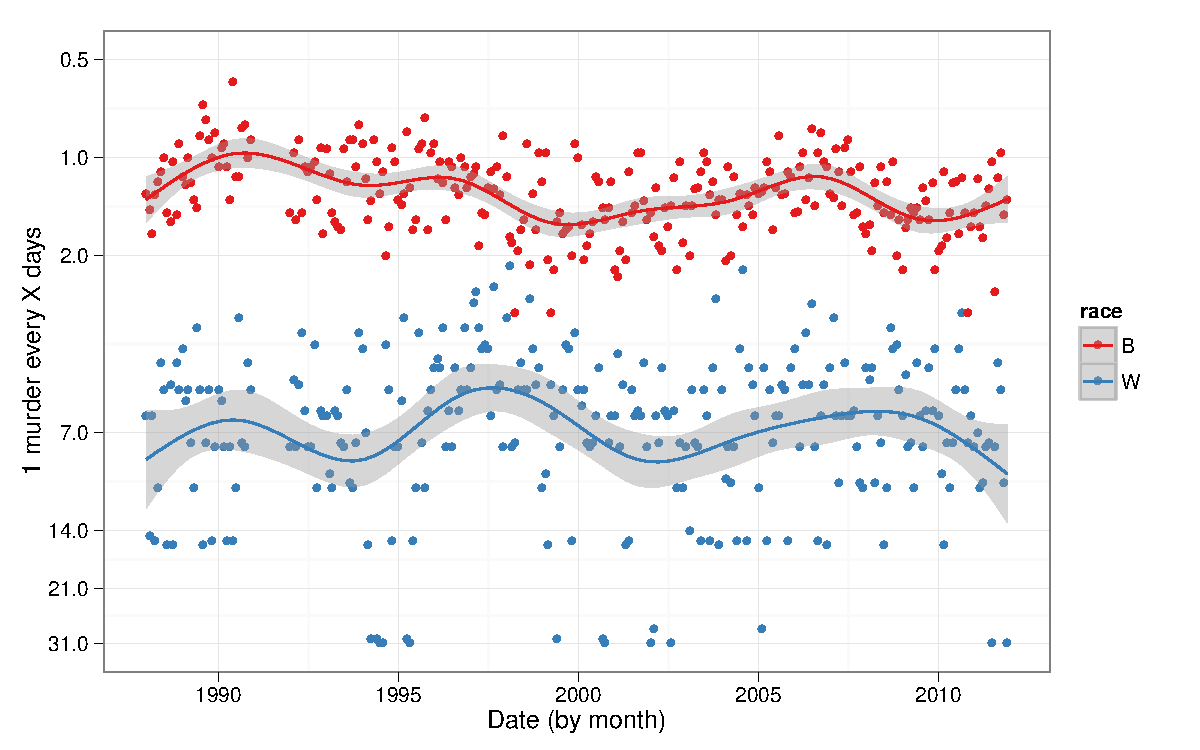
\includegraphics[width=\linewidth]{figures/murder-unnamed-chunk-9} 
\end{knitrout}

\end{frame}


\begin{frame}[fragile]
\frametitle{Two Philadelphias}

\begin{knitrout}
\definecolor{shadecolor}{rgb}{0.969, 0.969, 0.969}\color{fgcolor}\begin{kframe}
\begin{flushleft}
\ttfamily\noindent
\hlsymbol{model1}{\ }\hlassignement{\usebox{\hlnormalsizeboxlessthan}-}{\ }\hlfunctioncall{glm}\hlkeyword{(}\hlsymbol{freq}{\ }\hlkeyword{\urltilda{}}{\ }\hlsymbol{month}{\ }\hlkeyword{*}{\ }\hlsymbol{race}\hlkeyword{,}\hspace*{\fill}\\
\hlstd{}{\ }{\ }{\ }{\ }\hlargument{offset}{\ }\hlargument{=}{\ }\hlsymbol{ndays}\hlkeyword{,}{\ }\hlargument{family}{\ }\hlargument{=}{\ }\hlsymbol{poisson}\hlkeyword{,}{\ }\hlargument{data}{\ }\hlargument{=}{\ }\hlsymbol{philly.bw.count}\hlkeyword{)}\hspace*{\fill}\\
\hlstd{}\hlfunctioncall{anova}\hlkeyword{(}\hlsymbol{model1}\hlkeyword{,}{\ }\hlargument{test}{\ }\hlargument{=}{\ }\hlstring{"{}Chisq"{}}\hlkeyword{)}\mbox{}
\normalfont
\end{flushleft}
\begin{verbatim}
## Analysis of Deviance Table
## 
## Model: poisson, link: log
## 
## Response: freq
## 
## Terms added sequentially (first to last)
## 
## 
##            Df Deviance Resid. Df Resid. Dev Pr(>Chi)    
## NULL                         549       7593             
## month      11     2913       538       4680   <2e-16 ***
## race        1     3795       537        886   <2e-16 ***
## month:race 11        9       526        876     0.59    
## ---
## Signif. codes:  0 '***' 0.001 '**' 0.01 '*' 0.05 '.' 0.1 ' ' 1 
\end{verbatim}
\end{kframe}
\end{knitrout}


\end{frame}

\begin{frame}[fragile]
\frametitle{Two Philadelphias}






\begin{knitrout}
\definecolor{shadecolor}{rgb}{0.969, 0.969, 0.969}\color{fgcolor}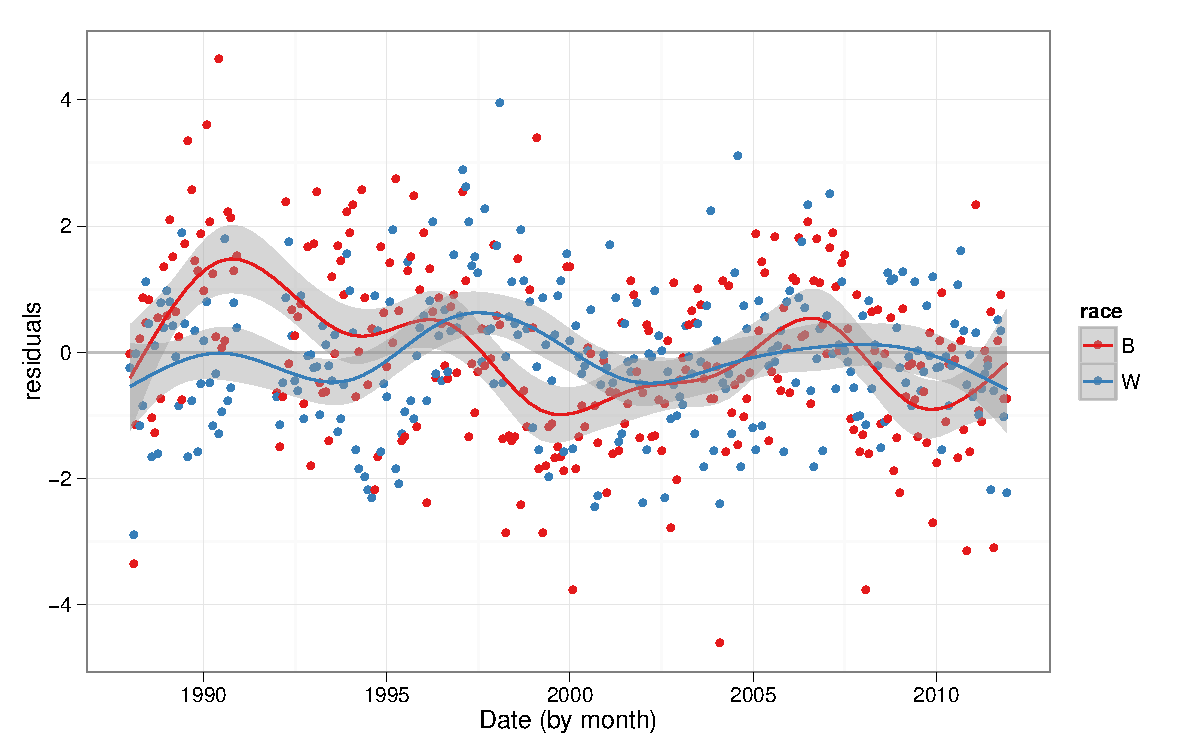
\includegraphics[width=\linewidth]{figures/murder-unnamed-chunk-12} 
\end{knitrout}

\end{frame}



\begin{frame}[fragile]
\frametitle{Two Philadelphias}
\begin{knitrout}
\definecolor{shadecolor}{rgb}{0.969, 0.969, 0.969}\color{fgcolor}\begin{kframe}
\begin{flushleft}
\ttfamily\noindent
\hlsymbol{philly.bw.count.w}{\ }\hlassignement{\usebox{\hlnormalsizeboxlessthan}-}{\ }\hlfunctioncall{count}\hlkeyword{(}\hlsymbol{philly.bw}\hlkeyword{,}\hspace*{\fill}\\
\hlstd{}{\ }{\ }{\ }{\ }\hlfunctioncall{c}\hlkeyword{(}\hlstring{"{}month.date"{}}\hlkeyword{,}{\ }\hlstring{"{}month"{}}\hlkeyword{,}{\ }\hlstring{"{}race"{}}\hlkeyword{,}{\ }\hlstring{"{}weapon"{}}\hlkeyword{,}\hspace*{\fill}\\
\hlstd{}{\ }{\ }{\ }{\ }{\ }{\ }{\ }{\ }\hlstring{"{}ndays"{}}\hlkeyword{)}\hlkeyword{)}\hspace*{\fill}\\
\hlstd{}\hlsymbol{philly.bw.count.w}{\ }\hlassignement{\usebox{\hlnormalsizeboxlessthan}-}{\ }\hlfunctioncall{transform}\hlkeyword{(}\hlsymbol{philly.bw.count.w}\hlkeyword{,}\hspace*{\fill}\\
\hlstd{}{\ }{\ }{\ }{\ }\hlargument{weapon}{\ }\hlargument{=}{\ }\hlfunctioncall{reorder}\hlkeyword{(}\hlsymbol{weapon}\hlkeyword{,}{\ }\hlkeyword{-}\hlsymbol{freq}\hlkeyword{,}{\ }\hlsymbol{sum}\hlkeyword{)}\hlkeyword{)}\hspace*{\fill}\\
\hlstd{}\hlsymbol{philly.bw.count.w}{\ }\hlassignement{\usebox{\hlnormalsizeboxlessthan}-}{\ }\hlfunctioncall{subset}\hlkeyword{(}\hlsymbol{philly.bw.count.w}\hlkeyword{,}\hspace*{\fill}\\
\hlstd{}{\ }{\ }{\ }{\ }\hlsymbol{weapon}{\ }\hlkeyword{\usebox{\hlnormalsizeboxpercent}in\usebox{\hlnormalsizeboxpercent}}{\ }\hlfunctioncall{c}\hlkeyword{(}\hlstring{"{}FIREARM"{}}\hlkeyword{,}{\ }\hlstring{"{}KNIFE"{}}\hlkeyword{,}{\ }\hlstring{"{}HANDS"{}}\hlkeyword{)}\hlkeyword{)}\hspace*{\fill}\\
\hlstd{}\hlfunctioncall{head}\hlkeyword{(}\hlsymbol{philly.bw.count.w}\hlkeyword{)}\mbox{}
\normalfont
\end{flushleft}
\begin{verbatim}
##   month.date month race  weapon ndays freq
## 1 1988-01-01   Jan    B FIREARM    31   13
## 2 1988-01-01   Jan    B   HANDS    31    7
## 3 1988-01-01   Jan    B   KNIFE    31    4
## 4 1988-01-01   Jan    W FIREARM    31    3
## 5 1988-01-01   Jan    W   KNIFE    31    1
## 7 1988-02-01   Feb    B FIREARM    29   11
\end{verbatim}
\end{kframe}
\end{knitrout}

\end{frame}


\begin{frame}[fragile]
\begin{knitrout}
\definecolor{shadecolor}{rgb}{0.969, 0.969, 0.969}\color{fgcolor}\begin{kframe}
\begin{flushleft}
\ttfamily\noindent
\hlcomment{\usebox{\hlnormalsizeboxhash}\usebox{\hlnormalsizeboxhash}{\ }To{\ }capture{\ }0{\ }counts}\hspace*{\fill}\\
\hlstd{}\hlsymbol{months.grid}{\ }\hlassignement{\usebox{\hlnormalsizeboxlessthan}-}{\ }\hlfunctioncall{expand.grid}\hlkeyword{(}\hlargument{month.date}{\ }\hlargument{=}{\ }\hlfunctioncall{unique}\hlkeyword{(}\hlsymbol{philly.bw}\hlkeyword{\usebox{\hlnormalsizeboxdollar}}\hlsymbol{month.date}\hlkeyword{)}\hlkeyword{,}\hspace*{\fill}\\
\hlstd{}{\ }{\ }{\ }{\ }\hlargument{race}{\ }\hlargument{=}{\ }\hlfunctioncall{c}\hlkeyword{(}\hlstring{"{}B"{}}\hlkeyword{,}{\ }\hlstring{"{}W"{}}\hlkeyword{)}\hlkeyword{,}{\ }\hlargument{weapon}{\ }\hlargument{=}{\ }\hlfunctioncall{c}\hlkeyword{(}\hlstring{"{}FIREARM"{}}\hlkeyword{,}\hspace*{\fill}\\
\hlstd{}{\ }{\ }{\ }{\ }{\ }{\ }{\ }{\ }\hlstring{"{}KNIFE"{}}\hlkeyword{,}{\ }\hlstring{"{}HANDS"{}}\hlkeyword{)}\hlkeyword{)}\hspace*{\fill}\\
\hlstd{}\hlsymbol{months.grid}{\ }\hlassignement{\usebox{\hlnormalsizeboxlessthan}-}{\ }\hlfunctioncall{join}\hlkeyword{(}\hlsymbol{months.grid}\hlkeyword{,}{\ }\hlsymbol{ndays}\hlkeyword{)}\hspace*{\fill}\\
\hlstd{}\hlsymbol{months.grid}\hlkeyword{\usebox{\hlnormalsizeboxdollar}}\hlsymbol{month}{\ }\hlassignement{\usebox{\hlnormalsizeboxlessthan}-}{\ }\hlsymbol{month.abb}\hlkeyword{[}\hlfunctioncall{as.POSIXlt}\hlkeyword{(}\hlsymbol{months.grid}\hlkeyword{\usebox{\hlnormalsizeboxdollar}}\hlsymbol{month.date}\hlkeyword{)}\hlkeyword{\usebox{\hlnormalsizeboxdollar}}\hlsymbol{mon}{\ }\hlkeyword{+}\hspace*{\fill}\\
\hlstd{}{\ }{\ }{\ }{\ }\hlnumber{1}\hlkeyword{]}\hspace*{\fill}\\
\hlstd{}\hspace*{\fill}\\
\hlstd{}\hlsymbol{philly.bw.count.w}{\ }\hlassignement{\usebox{\hlnormalsizeboxlessthan}-}{\ }\hlfunctioncall{merge}\hlkeyword{(}\hlsymbol{months.grid}\hlkeyword{,}\hspace*{\fill}\\
\hlstd{}{\ }{\ }{\ }{\ }\hlsymbol{philly.bw.count.w}\hlkeyword{,}{\ }\hlargument{all.x}{\ }\hlargument{=}{\ }\hlsymbol{T}\hlkeyword{)}\hspace*{\fill}\\
\hlstd{}\hlsymbol{philly.bw.count.w}\hlkeyword{\usebox{\hlnormalsizeboxdollar}}\hlsymbol{freq}\hlkeyword{[}\hlfunctioncall{is.na}\hlkeyword{(}\hlsymbol{philly.bw.count.w}\hlkeyword{\usebox{\hlnormalsizeboxdollar}}\hlsymbol{freq}\hlkeyword{)}\hlkeyword{]}{\ }\hlassignement{\usebox{\hlnormalsizeboxlessthan}-}{\ }\hlnumber{0}\mbox{}
\normalfont
\end{flushleft}
\end{kframe}
\end{knitrout}


\end{frame}

\begin{frame}
\frametitle{Two Philadelphias}



\begin{knitrout}
\definecolor{shadecolor}{rgb}{0.969, 0.969, 0.969}\color{fgcolor}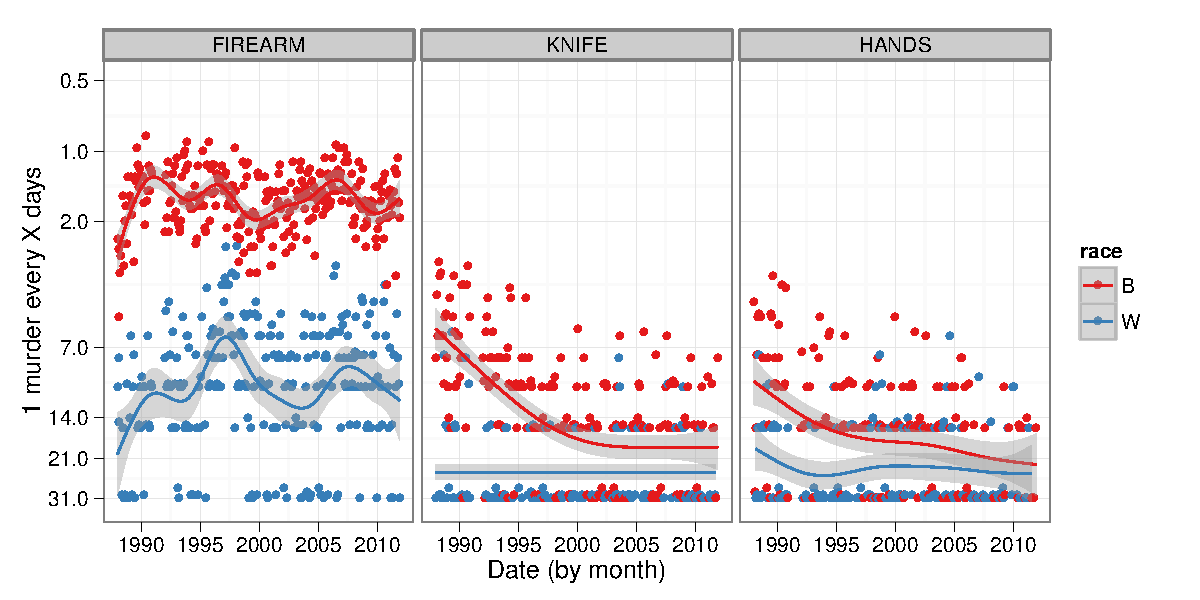
\includegraphics[width=\linewidth]{figures/murder-unnamed-chunk-15} 
\end{knitrout}

\end{frame}


\begin{frame}[fragile]
\begin{knitrout}
\definecolor{shadecolor}{rgb}{0.969, 0.969, 0.969}\color{fgcolor}\begin{kframe}
\begin{flushleft}
\ttfamily\noindent
\hlsymbol{model2}{\ }\hlassignement{\usebox{\hlnormalsizeboxlessthan}-}{\ }\hlfunctioncall{glm}\hlkeyword{(}\hlsymbol{freq}{\ }\hlkeyword{\urltilda{}}{\ }\hlsymbol{month}{\ }\hlkeyword{+}{\ }\hlsymbol{weapon}{\ }\hlkeyword{*}\hspace*{\fill}\\
\hlstd{}{\ }{\ }{\ }{\ }\hlsymbol{race}\hlkeyword{,}{\ }\hlargument{offset}{\ }\hlargument{=}{\ }\hlsymbol{ndays}\hlkeyword{,}{\ }\hlargument{data}{\ }\hlargument{=}{\ }\hlsymbol{philly.bw.count.w}\hlkeyword{,}\hspace*{\fill}\\
\hlstd{}{\ }{\ }{\ }{\ }\hlargument{family}{\ }\hlargument{=}{\ }\hlsymbol{poisson}\hlkeyword{)}\hspace*{\fill}\\
\hlstd{}\hlfunctioncall{anova}\hlkeyword{(}\hlsymbol{model2}\hlkeyword{,}{\ }\hlargument{test}{\ }\hlargument{=}{\ }\hlstring{"{}Chisq"{}}\hlkeyword{)}\mbox{}
\normalfont
\end{flushleft}
\begin{verbatim}
## Analysis of Deviance Table
## 
## Model: poisson, link: log
## 
## Response: freq
## 
## Terms added sequentially (first to last)
## 
## 
##             Df Deviance Resid. Df Resid. Dev Pr(>Chi)    
## NULL                         1655      16831             
## month       11     2841      1644      13990   <2e-16 ***
## weapon       2     7596      1642       6394   <2e-16 ***
## race         1     3766      1641       2628   <2e-16 ***
## weapon:race  2      116      1639       2512   <2e-16 ***
## ---
## Signif. codes:  0 '***' 0.001 '**' 0.01 '*' 0.05 '.' 0.1 ' ' 1 
\end{verbatim}
\end{kframe}
\end{knitrout}

\end{frame}

\begin{frame}
\frametitle{Two Philadelphias}
 \begin{itemize}
 	\item White murder victims are 
 		$5.71\times$ 
 		more likely to be shot than stabbed.
 	 	\item African American murder victims are 
 			$8.62\times$
 			more likely to be shot than stabbed.
 	\item African American murder victims are 
 			$1.51\times$
 			more likely to have been shot than White murder victims.
 \end{itemize}
\end{frame}






\begin{frame}
	\frametitle{Two Philadelphias}



\begin{knitrout}
\definecolor{shadecolor}{rgb}{0.969, 0.969, 0.969}\color{fgcolor}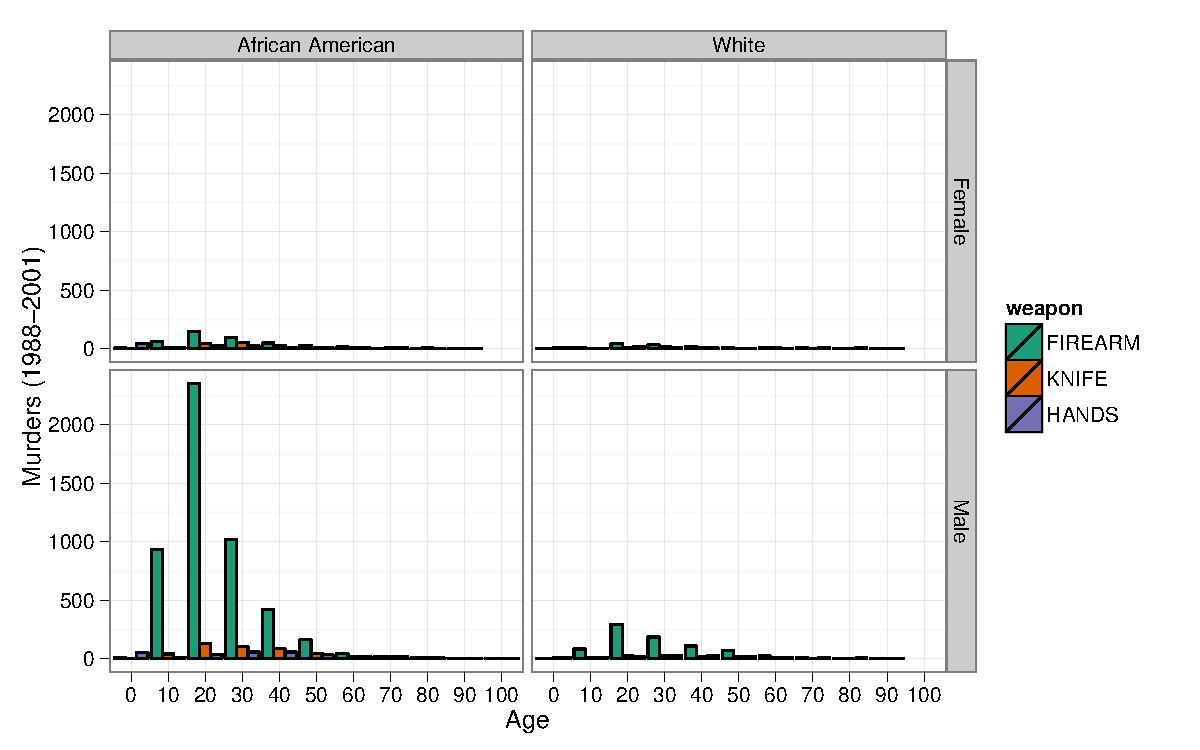
\includegraphics[width=\linewidth]{figures/murder-unnamed-chunk-18} 
\end{knitrout}


\end{frame}



\begin{frame}{}
	\begin{center}
		{\Huge Thanks}
	\end{center}
\end{frame}


\end{document}
